\chapter{Identificação do Túnel de Ar} \label{cap4}

\commentib{Todas as equações devem ser referenciadas com a função \texttt{eqref} ao invés de \texttt{ref}}

Neste capítulo \commentib{vírgula} será explicada a identificação do sistema do túnel de ar. Para fazer a identificação caixa-preta de um sistema é necessário fazer um estudo prévio do funcionamento dele, conhecer entradas e saídas, obter um modelo matemático se possível, mesmo sem ter todos os parâmetros.
\section{Escolha de estrutura}
A escolha da estrutura para identificar um sistema pode ser feita a partir de um modelagem prévia do sistema \commentib{Isso é parcialmente verdade, o conhecimento empírico da modelagem fenomeológica pode fornecer pistas sobre a estrutura, mas existem outros métodos que valem a pena ao menos serem citados, tais como análise de função de autocorrelação} , mas, em alguns casos a modelagem não é suficiente para obter um modelo adequado. O sistema estudado apresenta certos fenômenos físicos, como o giro da bola devido ao fluxo do ar, que não pudemos modelar.
\subsection{Mínimos Quadrados}\label{s:4mq}
A identificação por Mínimos Quadrados gera um sistema do típo ARX como visto na equação \ref{ARXModel}. A escolha da estrutura neste caso se dá escolhendo uma quantidade de regressores da saída e uma quantidade de regressores da entrada. Tendo em vista que o modelo matemático encontrado em \ref{eq:modelo} não é capaz de prever completamente o funcionamento do sistema foi necessário escolher um método diferente da análise do modelo \commentib{Essa última declaração deve ser melhorada. Pq não é capaz? E pq o modelo identificado é melhor?}.


Para a escolha da estrutura do modelo do sistema foi feito o seguinte procedimento:
\begin{enumerate}
	\item Escolher uma quantidade de regressores de $y$
	\item Escolher uma quantidade de regressores de $u$
	\item Fazer a identificação por Mínimos Quadrados com os regressores de $y$ e $u$
	\item Analisar a autocorrelação dos resíduos $\xi=y-\Psi \hat{\theta}$
\end{enumerate}

Este procedimento foi repetido para valores de 1 a 10 para ambos os regressores e ao final se identificou que a melhor ordem para os regressores foi com 9 polos e 8 zeros. Na figura \ref{fig:autocorrelacao98} a auto correlação dos resíduos do sistema identificado.


\commentib{Os testes de brancura/simula\c{c}\~oes devem ser expostos na seção de validação. Aqui você deve colocar apenas a estrutura.}

\begin{figure}[H]
	\centering
	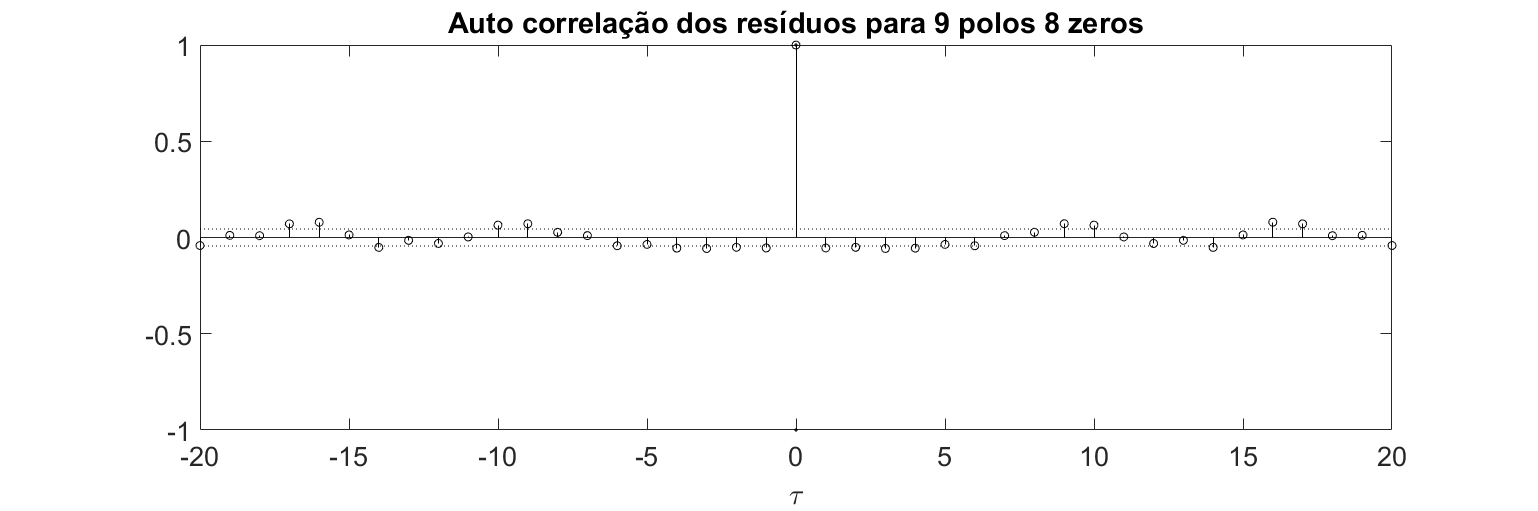
\includegraphics[width=1.1\linewidth]{autocorrelacao98}
	\caption[Autocorrelação dos resíduos para sistema com 9 polos e 8 zeros]{Autocorrelação dos resíduos para sistema com 9 polos e 8 zeros}
	\label{fig:autocorrelacao98}
\end{figure}

\subsection{Subespaços}\label{s:4subespacos}
A identificação por Subespaços gera um sistema em espaço de estados como visto na equação \ref{eq:ss}. Neste tipo de identificação a escolha da estrutura é feita decidindo a ordem do sistema e a ordem da matriz em blocos de Hankel. E similarmente ao procedimento feito na seção \ref{s:4mq} foram variadas as ordens do sistema e da matriz em blocos de Hankel.
Foi escolhida ordem 3 para o sistema e ordem 15 para a matriz em blocos de Hankel usada para identificar o sistema. Vemos na figura \ref{fig:autocorrelacao315} a auto correlação dos resíduos do sistema identificado.

\begin{figure}[H]
	\centering
	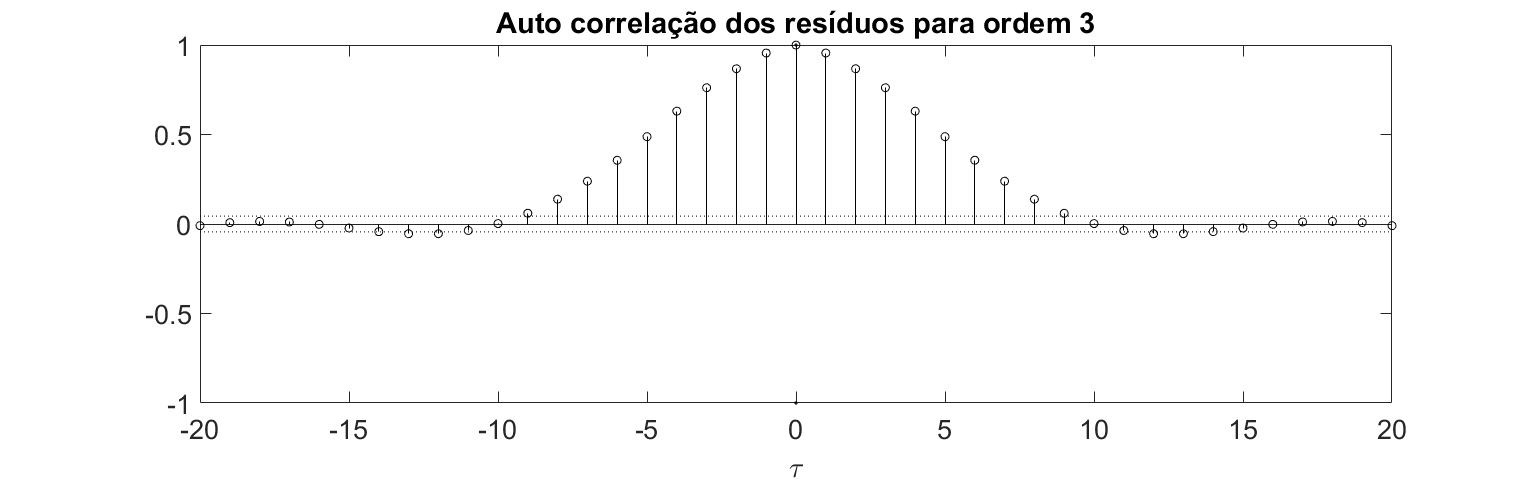
\includegraphics[width=1.1\linewidth]{autocorrelacao315}
	\caption[Autocorrelação dos resíduos para sistema de ordem 3]{Autocorrelação dos resíduos para sistema de ordem 3 identificado com matriz em blocos de Hankel ordem 15}
	\label{fig:autocorrelacao315}
\end{figure}

\section{Experimento}\label{s:4experimento}
O experimento para identificação precisa de um sinal adequado para que a resposta à ele consiga mostrar a dinâmica do sistema. Para tanto foi gerado um sinal PRBS (sinal binário pseudo aleatório) que é suficientemente adequado para extrair a dinâmica do sistema. O sinal é aplicado ao sistema através do Arduino e os sinais são medidos com um tempo de amostragem de 50 ms.
\begin{figure}[H]
	\centering
	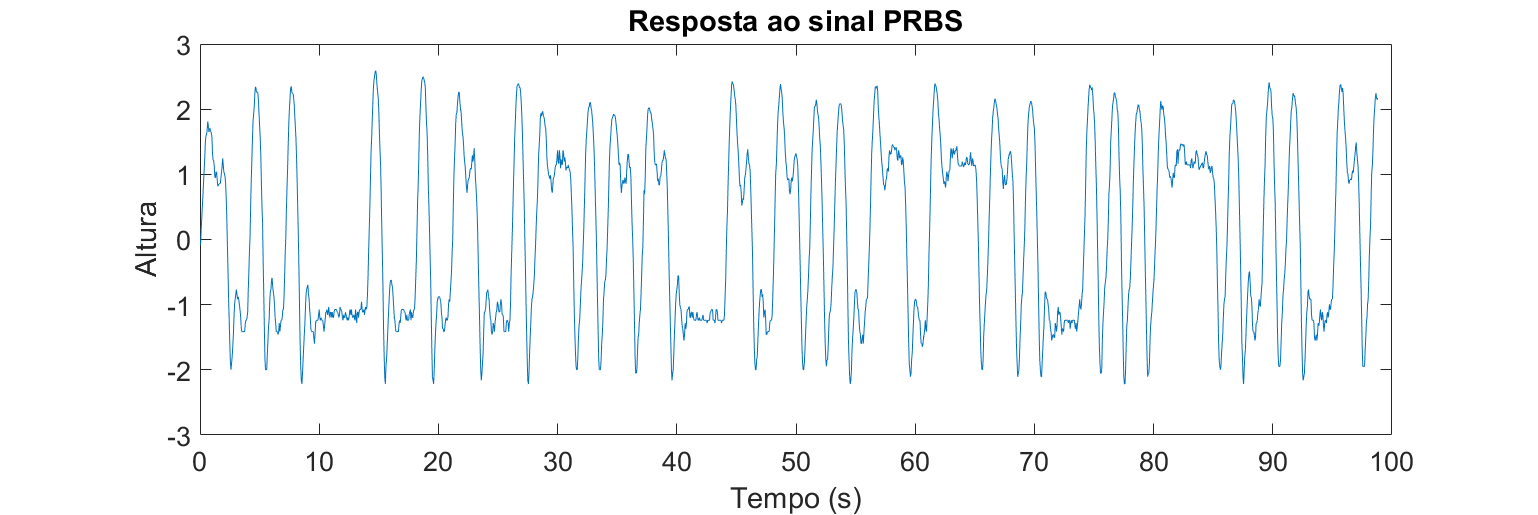
\includegraphics[width=1.1\linewidth]{sinalprbsid}
	\caption[Gráfico da saída PRBS]{Gráfico da saída ao aplicar o sinal PRBS com tempo de amostragem de 50ms}
	\label{fig:sinalprbsid}
\end{figure}

A figura \ref{fig:sinalprbsid} mostra a resposta do sistema ao sinal PRBS que foi aplicado ao sistema, podemos ver seções do teste onde o sinal possibilitou que o sistema tivesse algum tempo para estabilizar como em torno dos 10 e 80 segundos,e em outros o sistema é posto em movimento.

\section{Estimação}\label{s:4estimacao}

Com a resposta do sistema e o sinal de entrada podemos então identificar o sistema. \commentib{Fale mais...} 
\subsection{Mínimos Quadrados}\label{s:4estmq}
Para fazer a identificação por mínimos quadrados geramos a matriz de regressores $\psi$ da equação \ref{eq:regressores} e usamos a equação \ref{eq:MQ} para obter os coeficientes dos regressores. Obtemos um sistema com o seguinte modelo ARX:


\commentib{Se você explicitar a estrutura lá atrás, você pode apenas fornecer os parâmetros aqui.}
\begin{equation}
y[k]= A[k]+ B[k] 
\end{equation}
\begin{equation}
\begin{aligned}
A[k]=- 1.463\cdot U[k-1] + 0.6593 \cdot U[k-2] - 0.4703\cdot U[k-3] + 0.3195\cdot U[k-4] + 0.1436\cdot U[k-5]\\- 0.1106\cdot U[k-6] + 0.07184 \cdot U[k-7] - 0.0766\cdot U[k-8] + 0.02136 \cdot U[k-9]
\end{aligned}
\end{equation}
\begin{equation}
\begin{aligned}
B[k]=-0.004773\cdot U[k-1] - 0.002941\cdot U[k-2] + 0.01512\cdot U[k-3] + 0.01026\cdot U[k-4]\\ + 0.04134\cdot U[k-5] + 0.01709\cdot U[k-6] + 0.003757\cdot U[k-7]   + 0.0386 U[k-8]
\end{aligned}
\end{equation}

A resposta ao degrau do sistema identificado é visto na figura \ref{fig:respostadegrauarx}.

\begin{figure}[H]
	\centering
	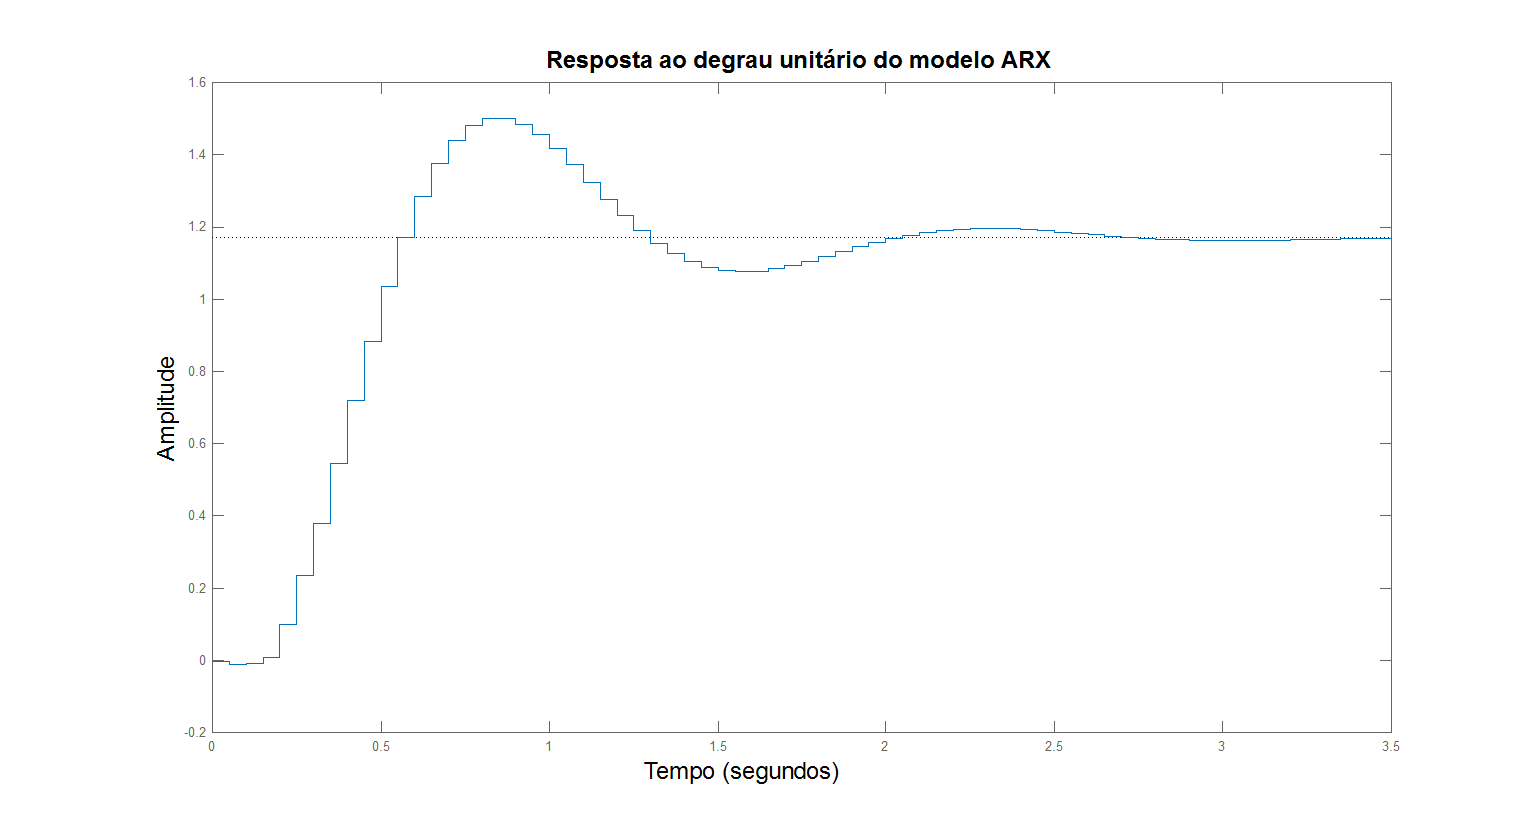
\includegraphics[width=1\linewidth]{respostadegrauarx}
	\caption[Resposta ao degrau do modelo ARX]{Resposta ao degrau unitário do modelo ARX identificado}
	\label{fig:respostadegrauarx}
\end{figure}

\subsection{Subespaços}\label{s:4estsub}

Para identificar o sistema usando subespaços utilizamos o algoritmo mostrado na seção \ref{s:subalgoritmos} com uma matriz em blocos de Hankel de ordem 15 para encontrar um sistema de ordem 3. Identificamos o seguinte modelo com o formato da equação \ref{eq:ss}:

\begin{equation}
A=\begin{bmatrix}
0.9761  &  0.1933 &  -0.0438\\
-0.1817  &  0.9841  & -0.1489\\
0.0840  &  0.3107  &  0.6994
\end{bmatrix}
\end{equation}

\begin{equation}
B=\begin{bmatrix}
0.1466\\
0.2515\\
0.8460
\end{bmatrix}
\end{equation}
\begin{equation}
C=\begin{bmatrix}
-1.0104 &  -0.3354 &   0.2496
\end{bmatrix}
\end{equation}
\begin{equation}
D=\begin{bmatrix}
0.0010
\end{bmatrix}
\end{equation}
Na figura \ref{fig:respostadegrausub} vemos a resposta ao degrau do sistema identificado, e, ao comparar com a resposta ao degrau do sistema ARX identificado, figura \ref{fig:respostadegrauarx}, podemos ver que ambos são sistemas estáveis e subamortecidos, apesar de apresentarem um tempo de assentamento diferente.

\begin{figure}[H]
	\centering
	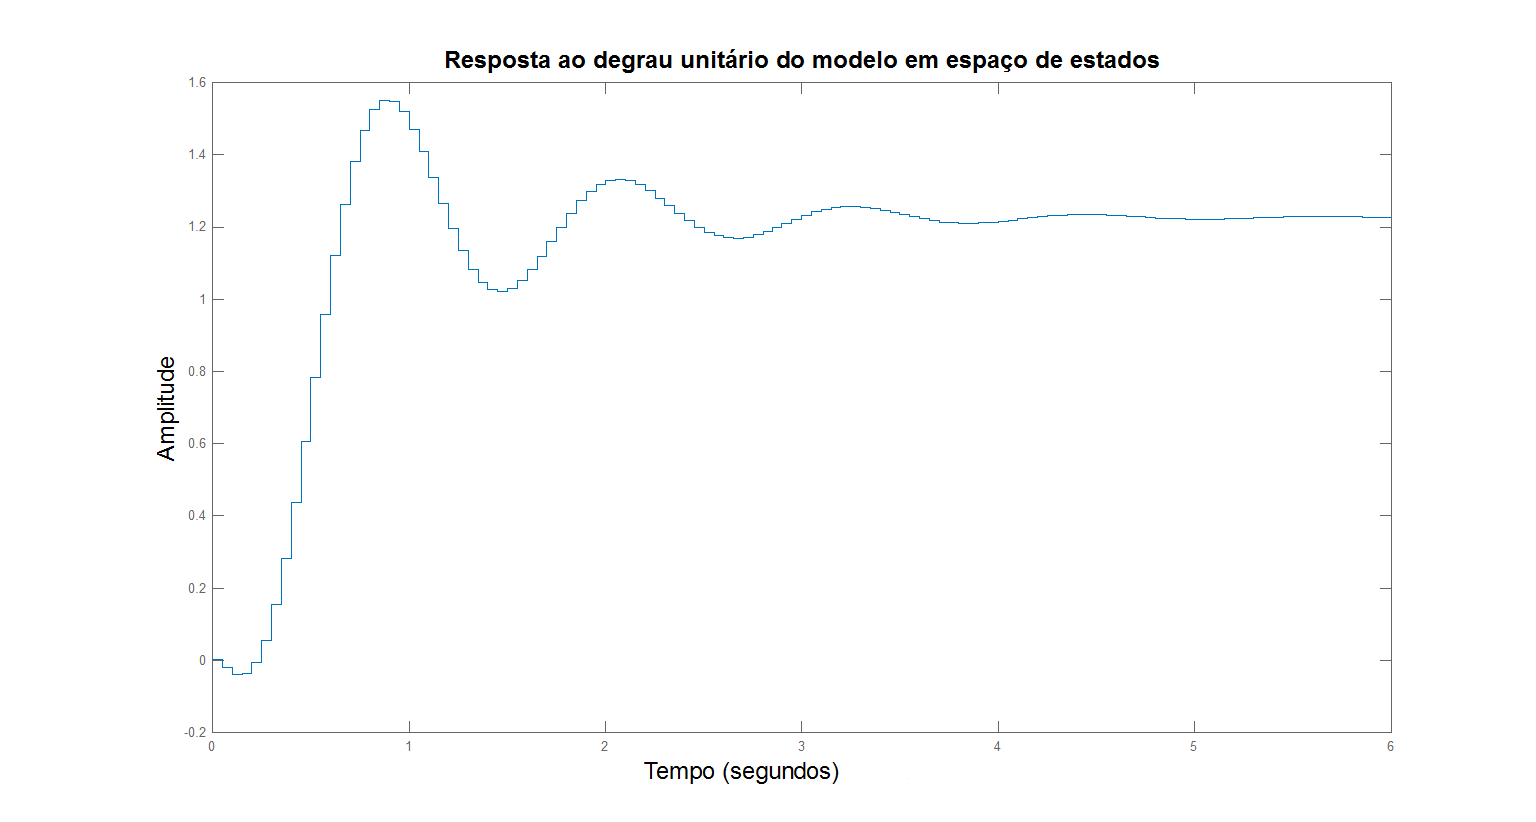
\includegraphics[width=1\linewidth]{respostadegrausub}
	\caption[Resposta ao degrau do modelo em espaço de estados]{Resposta ao degrau unitário do modelo em espaço de estados identificado}
	\label{fig:respostadegrausub}
\end{figure}

\section{Validação}\label{s4:val}
Ao identificar um sistema precisamos validar o modelo obtido para garantir que ele é adequado para representar o sistema real. Para isso fazemos uma análise da auto correlação dos resíduos $\xi=y-\Psi \hat{\theta}$ para o ARX e $\xi=y-y_{sim}$ para o espaço de estados. Como vemos nas figuras \ref{fig:autocorrelacao98} e \ref{fig:autocorrelacao315} os resíduos do modelo ARX são muito menos correlacionados do que os do modelo em espaço de estados. Isso acontece porque para o modelo ARX estamos analisando os seus regressores com a matriz $\Psi$ que os gera, o que retorna uma resposta muito mais próxima do sistema. Já para o espaço de estados estamos analisando a simulação do sistema, que apresenta pequenas diferenças em relação ao sistema real, como a ausência de ruído.


Ambos os sistemas, no entanto, apresentam uma análise de ruídos satisfatória e uma resposta ao sinal PRBS muito próxima do sistema real.



% Fim Capítulo